
%% bare_conf.tex
%% V1.3
%% 2007/01/11
%% by Michael Shell
%% See:
%% http://www.michaelshell.org/
%% for current contact information.
%%
%% This is a skeleton file demonstrating the use of IEEEtran.cls
%% (requires IEEEtran.cls version 1.7 or later) with an IEEE conference paper.
%%
%% Support sites:
%% http://www.michaelshell.org/tex/ieeetran/
%% http://www.ctan.org/tex-archive/macros/latex/contrib/IEEEtran/
%% and
%% http://www.ieee.org/

%%*************************************************************************
%% Legal Notice:
%% This code is offered as-is without any warranty either expressed or
%% implied; without even the implied warranty of MERCHANTABILITY or
%% FITNESS FOR A PARTICULAR PURPOSE! 
%% User assumes all risk.
%% In no event shall IEEE or any contributor to this code be liable for
%% any damages or losses, including, but not limited to, incidental,
%% consequential, or any other damages, resulting from the use or misuse
%% of any information contained here.
%%
%% All comments are the opinions of their respective authors and are not
%% necessarily endorsed by the IEEE.
%%
%% This work is distributed under the LaTeX Project Public License (LPPL)
%% ( http://www.latex-project.org/ ) version 1.3, and may be freely used,
%% distributed and modified. A copy of the LPPL, version 1.3, is included
%% in the base LaTeX documentation of all distributions of LaTeX released
%% 2003/12/01 or later.
%% Retain all contribution notices and credits.
%% ** Modified files should be clearly indicated as such, including  **
%% ** renaming them and changing author support contact information. **
%%
%% File list of work: IEEEtran.cls, IEEEtran_HOWTO.pdf, bare_adv.tex,
%%                    bare_conf.tex, bare_jrnl.tex, bare_jrnl_compsoc.tex
%%*************************************************************************

% *** Authors should verify (and, if needed, correct) their LaTeX system  ***
% *** with the testflow diagnostic prior to trusting their LaTeX platform ***
% *** with production work. IEEE's font choices can trigger bugs that do  ***
% *** not appear when using other class files.                            ***
% The testflow support page is at:
% http://www.michaelshell.org/tex/testflow/



% Note that the a4paper option is mainly intended so that authors in
% countries using A4 can easily print to A4 and see how their papers will
% look in print - the typesetting of the document will not typically be
% affected with changes in paper size (but the bottom and side margins will).
% Use the testflow package mentioned above to verify correct handling of
% both paper sizes by the user's LaTeX system.
%
% Also note that the "draftcls" or "draftclsnofoot", not "draft", option
% should be used if it is desired that the figures are to be displayed in
% draft mode.
%
\documentclass[conference]{IEEEtran}

\IEEEoverridecommandlockouts
% Add the compsoc option for Computer Society conferences.
%
% If IEEEtran.cls has not been installed into the LaTeX system files,
% manually specify the path to it like:
% \documentclass[conference]{../sty/IEEEtran}





% Some very useful LaTeX packages include:
% (uncomment the ones you want to load)


% *** MISC UTILITY PACKAGES ***
%
%\usepackage{ifpdf}
% Heiko Oberdiek's ifpdf.sty is very useful if you need conditional
% compilation based on whether the output is pdf or dvi.
% usage:
% \ifpdf
%   % pdf code
% \else
%   % dvi code
% \fi
% The latest version of ifpdf.sty can be obtained from:
% http://www.ctan.org/tex-archive/macros/latex/contrib/oberdiek/
% Also, note that IEEEtran.cls V1.7 and later provides a builtin
% \ifCLASSINFOpdf conditional that works the same way.
% When switching from latex to pdflatex and vice-versa, the compiler may
% have to be run twice to clear warning/error messages.






% *** CITATION PACKAGES ***
%
%\usepackage{cite}
% cite.sty was written by Donald Arseneau
% V1.6 and later of IEEEtran pre-defines the format of the cite.sty package
% \cite{} output to follow that of IEEE. Loading the cite package will
% result in citation numbers being automatically sorted and properly
% "compressed/ranged". e.g., [1], [9], [2], [7], [5], [6] without using
% cite.sty will become [1], [2], [5]--[7], [9] using cite.sty. cite.sty's
% \cite will automatically add leading space, if needed. Use cite.sty's
% noadjust option (cite.sty V3.8 and later) if you want to turn this off.
% cite.sty is already installed on most LaTeX systems. Be sure and use
% version 4.0 (2003-05-27) and later if using hyperref.sty. cite.sty does
% not currently provide for hyperlinked citations.
% The latest version can be obtained at:
% http://www.ctan.org/tex-archive/macros/latex/contrib/cite/
% The documentation is contained in the cite.sty file itself.






% *** GRAPHICS RELATED PACKAGES ***
%
\ifCLASSINFOpdf
  % \usepackage[pdftex]{graphicx}
  % declare the path(s) where your graphic files are
  % \graphicspath{{../pdf/}{../jpeg/}}
  % and their extensions so you won't have to specify these with
  % every instance of \includegraphics
  % \DeclareGraphicsExtensions{.pdf,.jpeg,.png}
\else
  % or other class option (dvipsone, dvipdf, if not using dvips). graphicx
  % will default to the driver specified in the system graphics.cfg if no
  % driver is specified.
  % \usepackage[dvips]{graphicx}
  % declare the path(s) where your graphic files are
  % \graphicspath{{../eps/}}
  % and their extensions so you won't have to specify these with
  % every instance of \includegraphics
  % \DeclareGraphicsExtensions{.eps}
\fi
% graphicx was written by David Carlisle and Sebastian Rahtz. It is
% required if you want graphics, photos, etc. graphicx.sty is already
% installed on most LaTeX systems. The latest version and documentation can
% be obtained at: 
% http://www.ctan.org/tex-archive/macros/latex/required/graphics/
% Another good source of documentation is "Using Imported Graphics in
% LaTeX2e" by Keith Reckdahl which can be found as epslatex.ps or
% epslatex.pdf at: http://www.ctan.org/tex-archive/info/
%
% latex, and pdflatex in dvi mode, support graphics in encapsulated
% postscript (.eps) format. pdflatex in pdf mode supports graphics
% in .pdf, .jpeg, .png and .mps (metapost) formats. Users should ensure
% that all non-photo figures use a vector format (.eps, .pdf, .mps) and
% not a bitmapped formats (.jpeg, .png). IEEE frowns on bitmapped formats
% which can result in "jaggedy"/blurry rendering of lines and letters as
% well as large increases in file sizes.
%
% You can find documentation about the pdfTeX application at:
% http://www.tug.org/applications/pdftex





% *** MATH PACKAGES ***
%
%\usepackage[cmex10]{amsmath}
% A popular package from the American Mathematical Society that provides
% many useful and powerful commands for dealing with mathematics. If using
% it, be sure to load this package with the cmex10 option to ensure that
% only type 1 fonts will utilized at all point sizes. Without this option,
% it is possible that some math symbols, particularly those within
% footnotes, will be rendered in bitmap form which will result in a
% document that can not be IEEE Xplore compliant!
%
% Also, note that the amsmath package sets \interdisplaylinepenalty to 10000
% thus preventing page breaks from occurring within multiline equations. Use:
%\interdisplaylinepenalty=2500
% after loading amsmath to restore such page breaks as IEEEtran.cls normally
% does. amsmath.sty is already installed on most LaTeX systems. The latest
% version and documentation can be obtained at:
% http://www.ctan.org/tex-archive/macros/latex/required/amslatex/math/





% *** SPECIALIZED LIST PACKAGES ***
%
%\usepackage{algorithmic}
% algorithmic.sty was written by Peter Williams and Rogerio Brito.
% This package provides an algorithmic environment fo describing algorithms.
% You can use the algorithmic environment in-text or within a figure
% environment to provide for a floating algorithm. Do NOT use the algorithm
% floating environment provided by algorithm.sty (by the same authors) or
% algorithm2e.sty (by Christophe Fiorio) as IEEE does not use dedicated
% algorithm float types and packages that provide these will not provide
% correct IEEE style captions. The latest version and documentation of
% algorithmic.sty can be obtained at:
% http://www.ctan.org/tex-archive/macros/latex/contrib/algorithms/
% There is also a support site at:
% http://algorithms.berlios.de/index.html
% Also of interest may be the (relatively newer and more customizable)
% algorithmicx.sty package by Szasz Janos:
% http://www.ctan.org/tex-archive/macros/latex/contrib/algorithmicx/




% *** ALIGNMENT PACKAGES ***
%
%\usepackage{array}
% Frank Mittelbach's and David Carlisle's array.sty patches and improves
% the standard LaTeX2e array and tabular environments to provide better
% appearance and additional user controls. As the default LaTeX2e table
% generation code is lacking to the point of almost being broken with
% respect to the quality of the end results, all users are strongly
% advised to use an enhanced (at the very least that provided by array.sty)
% set of table tools. array.sty is already installed on most systems. The
% latest version and documentation can be obtained at:
% http://www.ctan.org/tex-archive/macros/latex/required/tools/
\usepackage{amsmath}

%\usepackage{mdwmath}
%\usepackage{mdwtab}
% Also highly recommended is Mark Wooding's extremely powerful MDW tools,
% especially mdwmath.sty and mdwtab.sty which are used to format equations
% and tables, respectively. The MDWtools set is already installed on most
% LaTeX systems. The lastest version and documentation is available at:
% http://www.ctan.org/tex-archive/macros/latex/contrib/mdwtools/


% IEEEtran contains the IEEEeqnarray family of commands that can be used to
% generate multiline equations as well as matrices, tables, etc., of high
% quality.


%\usepackage{eqparbox}
% Also of notable interest is Scott Pakin's eqparbox package for creating
% (automatically sized) equal width boxes - aka "natural width parboxes".
% Available at:
% http://www.ctan.org/tex-archive/macros/latex/contrib/eqparbox/





% *** SUBFIGURE PACKAGES ***
%\usepackage[tight,footnotesize]{subfigure}
% subfigure.sty was written by Steven Douglas Cochran. This package makes it
% easy to put subfigures in your figures. e.g., "Figure 1a and 1b". For IEEE
% work, it is a good idea to load it with the tight package option to reduce
% the amount of white space around the subfigures. subfigure.sty is already
% installed on most LaTeX systems. The latest version and documentation can
% be obtained at:
% http://www.ctan.org/tex-archive/obsolete/macros/latex/contrib/subfigure/
% subfigure.sty has been superceeded by subfig.sty.



%\usepackage[caption=false]{caption}
%\usepackage[font=footnotesize]{subfig}
% subfig.sty, also written by Steven Douglas Cochran, is the modern
% replacement for subfigure.sty. However, subfig.sty requires and
% automatically loads Axel Sommerfeldt's caption.sty which will override
% IEEEtran.cls handling of captions and this will result in nonIEEE style
% figure/table captions. To prevent this problem, be sure and preload
% caption.sty with its "caption=false" package option. This is will preserve
% IEEEtran.cls handing of captions. Version 1.3 (2005/06/28) and later 
% (recommended due to many improvements over 1.2) of subfig.sty supports
% the caption=false option directly:
%\usepackage[caption=false,font=footnotesize]{subfig}
%
% The latest version and documentation can be obtained at:
% http://www.ctan.org/tex-archive/macros/latex/contrib/subfig/
% The latest version and documentation of caption.sty can be obtained at:
% http://www.ctan.org/tex-archive/macros/latex/contrib/caption/




% *** FLOAT PACKAGES ***
%
%\usepackage{fixltx2e}
% fixltx2e, the successor to the earlier fix2col.sty, was written by
% Frank Mittelbach and David Carlisle. This package corrects a few problems
% in the LaTeX2e kernel, the most notable of which is that in current
% LaTeX2e releases, the ordering of single and double column floats is not
% guaranteed to be preserved. Thus, an unpatched LaTeX2e can allow a
% single column figure to be placed prior to an earlier double column
% figure. The latest version and documentation can be found at:
% http://www.ctan.org/tex-archive/macros/latex/base/



%\usepackage{stfloats}
% stfloats.sty was written by Sigitas Tolusis. This package gives LaTeX2e
% the ability to do double column floats at the bottom of the page as well
% as the top. (e.g., "\begin{figure*}[!b]" is not normally possible in
% LaTeX2e). It also provides a command:
%\fnbelowfloat
% to enable the placement of footnotes below bottom floats (the standard
% LaTeX2e kernel puts them above bottom floats). This is an invasive package
% which rewrites many portions of the LaTeX2e float routines. It may not work
% with other packages that modify the LaTeX2e float routines. The latest
% version and documentation can be obtained at:
% http://www.ctan.org/tex-archive/macros/latex/contrib/sttools/
% Documentation is contained in the stfloats.sty comments as well as in the
% presfull.pdf file. Do not use the stfloats baselinefloat ability as IEEE
% does not allow \baselineskip to stretch. Authors submitting work to the
% IEEE should note that IEEE rarely uses double column equations and
% that authors should try to avoid such use. Do not be tempted to use the
% cuted.sty or midfloat.sty packages (also by Sigitas Tolusis) as IEEE does
% not format its papers in such ways.





% *** PDF, URL AND HYPERLINK PACKAGES ***
%
%\usepackage{url}
% url.sty was written by Donald Arseneau. It provides better support for
% handling and breaking URLs. url.sty is already installed on most LaTeX
% systems. The latest version can be obtained at:
% http://www.ctan.org/tex-archive/macros/latex/contrib/misc/
% Read the url.sty source comments for usage information. Basically,
% \url{my_url_here}.


\usepackage[utf8]{inputenc}
\usepackage{graphicx}


% *** Do not adjust lengths that control margins, column widths, etc. ***
% *** Do not use packages that alter fonts (such as pslatex).         ***
% There should be no need to do such things with IEEEtran.cls V1.6 and later.
% (Unless specifically asked to do so by the journal or conference you plan
% to submit to, of course. )


% correct bad hyphenation here
\hyphenation{op-tical net-works semi-conduc-tor}


\begin{document}

%
% paper title
% can use linebreaks \\ within to get better formatting as desired
\title{Software Defined Networking for RSU Clouds in support of The Internet of Vehicles}


% author names and affiliations
% use a multiple column layout for up to three different
% affiliations
\author{\IEEEauthorblockN{Christoph Wittmann}
\IEEEauthorblockA{Lehrstuhl für Kommunikationsnetze\\
Technische Universität München\\
80333 München\\
Email: christoph.wittmann@tum.de}
%\and
%\IEEEauthorblockN{Your supervisor is NOT! an author of your paper!}
%\IEEEauthorblockA{Starfleet Academy\\
%San Francisco, California 96678-2391\\
%Telephone: (800) 555--1212\\
%Fax: (888) 555--1212}

\thanks{*This paper is a reinterpretation of the paper \emph{M.A. Salahuddin. ``Software Defined Networking for RSU Clouds in support of The Internet of Vehicles,'' Internet of Things Journal, IEEE, 2014, pp. 133-144}. It was presented on June 22, 2015 (Paper submission deadline) as a part of MSCE Seminar (MSCE course TUM), under the supervision of M. Sc. 
Christian Sieber (c.sieber@tum.de).}
}

% conference papers do not typically use \thanks and this command
% is locked out in conference mode. If really needed, such as for
% the acknowledgment of grants, issue a \IEEEoverridecommandlockouts
% after \documentclass

% for over three affiliations, or if they all won't fit within the width
% of the page, use this alternative format:
% 
%\author{\IEEEauthorblockN{Michael Shell\IEEEauthorrefmark{1},
%Homer Simpson\IEEEauthorrefmark{2},
%James Kirk\IEEEauthorrefmark{3}, 
%Montgomery Scott\IEEEauthorrefmark{3} and
%Eldon Tyrell\IEEEauthorrefmark{4}}
%\IEEEauthorblockA{\IEEEauthorrefmark{1}School of Electrical and Computer Engineering\\
%Georgia Institute of Technology,
%Atlanta, Georgia 30332--0250\\ Email: see http://www.michaelshell.org/contact.html}
%\IEEEauthorblockA{\IEEEauthorrefmark{2}Twentieth Century Fox, Springfield, USA\\
%Email: homer@thesimpsons.com}
%\IEEEauthorblockA{\IEEEauthorrefmark{3}Starfleet Academy, San Francisco, California 96678-2391\\
%Telephone: (800) 555--1212, Fax: (888) 555--1212}
%\IEEEauthorblockA{\IEEEauthorrefmark{4}Tyrell Inc., 123 Replicant Street, Los Angeles, California 90210--4321}}




% use for special paper notices
%\IEEEspecialpapernotice{(Invited Paper)}




% make the title area
\maketitle


\begin{abstract}
%\boldmath

\end{abstract}
% IEEEtran.cls defaults to using nonbold math in the Abstract.
% This preserves the distinction between vectors and scalars. However,
% if the conference you are submitting to favors bold math in the abstract,
% then you can use LaTeX's standard command \boldmath at the very start
% of the abstract to achieve this. Many IEEE journals/conferences frown on
% math in the abstract anyway.

% no keywords




% For peer review papers, you can put extra information on the cover
% page as needed:
% \ifCLASSOPTIONpeerreview
% \begin{center} \bfseries EDICS Category: 3-BBND \end{center}
% \fi
%
% For peerreview papers, this IEEEtran command inserts a page break and
% creates the second title. It will be ignored for other modes.
\IEEEpeerreviewmaketitle



\section{Einleitung}
% no \IEEEPARstart

Intelligente Transport Systeme sind die Zukunft unserer Schienen, Straßen sowie Luft-und Wasserwege und ein großes aktuelles Forschungsgebiet. Durch die damit einhergehende Zusammenführung von Transport und Kommunikation wird sich ein großes Plus in Sachen Sicherheit, Effizienz und Ökologie versprochen. Dies soll unter anderem durch intelligente Ausbalancierung des Verkehrs zur Stauvermeidung oder durch die Warnung vor potentiellen Gefahrenstellen in Echtzeit erreicht werden. Gerade im Straßenverkehr werden jedoch von den Verkehrsteilnehmern auch immer mehr Dienste zur Unterhaltung, wie zum Beispiel Video Streaming, mobiles Internet und Internettelefonie nachgefragt. Diese Nachfrage an bandbreitenhungrigen Anwendungen stellen große Anforderungen an ein Kommunikationsnetz. Hinzu kommt, dass sich der Bedarf an Ressourcen durch die naturgemäß hohe Mobilität der Verkehrskehrsteilnehmer dynamisch ändert. Die Ressourcen müssen in der Regel bei einem Dienstleister angemietet werden und verursachen Kosten für einen Dienstanbieter. Um diese Kosten zu minimieren erfordert dies in der Praxis eine ständige bedarfsgerechte Umverteilung der Ressourcen  und eine damit verbundene Neukonfiguration des Kommunikationsnetzes. Einen Lösungsansatz für diese Problemstellung hat Salahuddin et al. in einem Paper mit dem Titel: "Software Defined Networking for RSU Clouds in support of The Internet of Vehicles" vorgestellt. Dort wird eine neuartige Cloud Architektur beschrieben, die durch das Ausnutzen der Vorteile von SDN in hohem Maße flexibel konfigurierbar ist. Konkret bedeutet das, dass innerhalb der Cloud einzelne Dienste verschoben oder an einen anderen Ort kopiert werden, um der wechselnden Nachfrage gerecht zu werden.\\
Mein eigener Beitrag ist die Zusammenfassung der in diesem Paper vorgestellten Cloud sowie die Ergänzung durch relevante Hintergrundinformationen wie SDN oder die Darstellung anderer Ansätze.\\
Dieses Paper gliedert sich wie folgt. Im Abschnitt II wird eine kurze Einführung in SDN und dessen Eigenschaften gegeben. In Abschnitt III finden sich eine Darstellung des Aufbaus einer RSU Cloud und deren Komponenten sowie die Anforderungen, die an eine RSU Cloud gestellt werden. Andere Ansätze und deren Vor- und Nachteile werden in Abschnitt IV erläutert. In Abschnitt V werden das Modell zum Ressourcen Management in der Cloud vorgestellt.  In Abschnitt VI werden die Ergebnisse der Simulationen präsentiert und mit anderen Ansätzen verglichen. Abschließend werde ich in Abschnitt VII die Ergebnisse zusammenfassen und einen Ausblick auf weiterführende Arbeit geben.




% You must have at least 2 lines in the paragraph with the drop letter
% (should never be an issue)


\section{Einführung in Software Defined Networking (SDN)}

In diesem Kapitel wird ein Überblick über das Themengebiet Software Defined Networking gegeben und die elementaren Eigenschaften des Konzepts dargelegt. Ziel dieses Kapitels ist es, die zum Verständnis notwenigen Hintergrundinformationen zu SDN zusammenzufassen und das Bewusstsein dafür zu schärfen, was SDN eigentlich ausmacht.  Um eine Technologie als SDN zu bezeichnen müssen laut [1] vier Prinzipien erfüllt sein, die ich im Folgenden kurz zusammenfassen möchte. Der zentrale Grundsatz in SDN ist die Trennung des Netzwerks in eine physikalische Datenebene und eine davon abstrahierte Kontrollebene. Das bedeutet, dass in einer SDN-fähigen Netzwerkkomponente eine von der Datenebene abgekoppelte, externe Instanz existieren muss. Diese Instanz wird Controller genannt und zeichnet sich dadurch aus, dass sie die Möglichkeit hat, das Weiterleitungsverhalten einer Netzwerkkomponente direkt zu bestimmen. In der Praxis besteht ein SDN daher aus Controllern und Switches. In einem Switch sind nur noch die, von ihm auszuführenden Weiterleitungsvorschriften gespeichert, die dynamisch von einem Controller über die Kontrollebene aktualisiert werden können.  Daraus ergibt sich zum Beispiel der Vorteil, dass Daten- und Kontrollebene im Design beziehungsweise in Untersuchungen und Analysen getrennt voneinander betrachtet werden können. \\
Ein weiteres Prinzip ist, dass ein derartiger Controller, obwohl er sich in einem SDN Netzwerk auf mehrere virtuelle oder physikalische Bestandteile verteilen kann, sich trotzdem logisch wie eine zentrale Einheit verhält, die über globales Wissen verfügt. Diese Eigenschaft bringt den Vorteil der schnelleren und effizienteren dynamischen Anpassung des Netzwerks.
Als dritten Grundsatz wird in [1] die Offenheit der Schnittstellen genannt, worauf ich hier aber aus Relevanzgründen nicht näher eingehen möchte. Viel interessanter ist die Eigenschaft der Programmierbarkeit eines SDN Netzes. Dies wird durch die Entkopplung von Daten- und Kontrollebene ermöglicht und macht das Netzwerk extrem anpassbar an verschiedene Anwendungen. Laut [1] lässt sich das Netzwerk dann als eine einzige programmierbare Einheit behandeln und nicht als eine Anhäufung von Geräten, die individuell konfiguriert werden müssen.\\
OpenFlow ist das am weitesten verbreitete Kommunikationsprotokoll, das in SDN eingesetzt wird. Es fungiert als Schnittstelle zwischen Datenebene und Kontrollebene, indem es direkten Zugriff auf Weiterleitungsverhalten eines Switches ermöglicht. Man spricht daher auch häufig von OpenFlow Kontrollern oder OpenFlow Switches. 


\section{Architektur der RSU Cloud}

Ein Fahrzeugnetzwerk (Vehicular Grid) besteht grob aus zwei Arten von Komponenten. Auf der einen Seite sind das Lokalisierungssysteme, Sensoren, Mikroprozessoren und Funkeinheiten, die an einem Fahrzeug montiert sind - sogenannte On-Board Units(OBUs) - und auf der anderen Seite  Sensoren und Mikrocontroller, die fest in die Straßen integriert sind, genannt Roadside Units(RSUs). Diese Komponenten vernetzt bilden ein sogenanntes Fahrzeug Ad hoc Netzwerk (VANET).  Der neue Ansatz, der in diesem Paper diskutiert wird, ist die Zusammenfassung der RSUs zu einer RSU Cloud.\\
Da eine derartige Cloud demnach alle nachgefragten Sicherheits- sowie Unterhaltungsdienste bereitstellen können muss, werden hohe Anforderungen an sie gestellt. Eine RSU Cloud muss nicht nur verlässlich sondern auch sehr leistungsstark in Sachen Datenrate und Latenz sein, um größtmögliche Sicherheit zu garantieren und somit die Akzeptanz in der Bevölkerung zu erlangen.\\
Eine solche RSU Cloud besteht dabei neben gewöhnlichen RSUs zudem aus RSU Mikrodatenzentren. Ein Mikrodatenzentrum besteht aus einer kleinen Recheneinheit und einem OpenFlow Switch, sodass es in ein SDN Netzwerk eingebunden werden kann. Softwareseitig besteht ein Mikrodatenzentrum aus einem Betriebssystem und einem Hypervisor, der es mittels Virtualisierung ermöglicht mehrere virtuelle Maschinen dynamisch auf einem Host auszuführen. Auf einem solchen Mikrodatenzentrum sollen dann die Dienste gehostet werden, die von den Verkehrsteilnehmern nachgefragt werden. Dies hat den großen Vorteil, dass die Dienste sehr "nah" an den Konsumenten sind, was sich in einer höheren Verlässlichkeit und kürzeren Latenzzeiten bemerkbar macht. Die, zum Aufspannen einer Cloud in einem SDN Netzwerk, nötigen Softwarekomponenten wie ein OpenFlow Controller oder ein Cloud Kontroller sollen ebenfalls in manchen Mikrodatenzentren ausgeführt werden. Eine weitere neue Komponente, die im Originalpaper vorgestellt wurde, ist der RSU Cloud Resource Manager(CRM). Der CRM ist ebenfalls in manchen Mikrodatenzentren integriert und soll Informationen über das Hosten von Diensten, die Verschiebung von Diensten oder das Ändern von Weiterleitungsvorschriften verbreiten, indem er mit OpenFlow und Cloud Kontrollern kommuniziert. Des Weiteren hat er die Aufgabe, die richtigen Entscheidungen bezüglich der optimalen Lage und Anzahl an gehosteten Diensten und den dazugehörigen Weiterleitungsvorschriften zu treffen. Entscheidend ist hierbei, dass die Anzahl an Verschiebungen von virtuellen Maschinen möglichst gering gehalten wird, da sie zusätzlichen Netzwerkverkehr in Daten und Kontrollebene produzieren und somit negativen Einfluss auf Quality of Service und darüber hinaus auch zusätzliche Kosten für den Anbieter eines Dienstes haben. Im Weiteren soll nun die Formalisierung des zusätzlichen Netzwerkverkehrs, der durch eine Neukonfiguration des Netzes entsteht, beschrieben werden. Zunächst einmal ist der Begriff der Konfiguration einzuführen, der den Zustand des Netzes zum Zeitpunkt \(t_i\) beschreibt. Eine Konfiguration ist somit definiert als 3-Tupel \(<X^{t_i},Y^{t_i},Z^{t_i}>\) mit den Komponenten $X^{t_i}$  welche den Satz an Hosts darstellt, \(Y^{t_i}\)  die den Satz an Weiterleitungsvorschriften repräsentiert und \(Z^{t_i}\),  dem Satz an Vorschriften für die Weiterleitung eines Eingangs an mehrere Empfänger, den sogenannten Gruppenvorschriften. Zur Bestimmung des verursachten Netzverkehrs in der Datenebene werden nun die Verschiebungen von Diensten gezählt. Formal kann man die Verschiebungen vom Zeitpunkt \(t_i\) zum Zeitpunkt \(t_{i+1}\) mit der Formel \(|X^{t_i}-X^{t_{i+1}}|\) ausdrücken. Ein Spezialfall ist hier das Löschen eines Dienstes von einem Host, was nicht berücksichtigt wird, da kein Datenaustausch auf der Datenebene erforderlich ist. Für die Analyse des Verkehrs in der Kontrollebene werden die Veränderungen der Weiterleitungs- und Gruppenvorschriften herangezogen. Der Verkehr setzt sich hier aus der Summe der Weiterleitungs-beziehungsweise Gruppenvorschriften, die hinzugefügt oder gelöscht werden und außerdem aus der Anzahl der Weiterleitungsvorschriften die zu Gruppenvorschriften und der Gruppenregeln die zu Weiterleitungsvorschriften werden, zusammen. Daraus ergibt sich folgende Formel für den zusätzlichen Verkehr in der Kontrollebene:  \(|Y^{t_i}-Y^{t_{i+1}}|+|Y^{t_{i+1}}-Y^{t_{i}}|+|Z^{t_i}-Z^{t_{i+1}}|+|Z^{t_{i+1}}-Z^{t_{i}}|+|Y^{t_i} \cap Z^{t_{i+1}}|+|Z^{t_{i}} \cap Y^{t_{i+1}}|\).



\section{"related Work" oder Hintergrund(siehe III. Background)}
\begin{itemize}
\item Darlegung anderer Ansätze und deren Vor- und Nachteile
\begin{itemize}
\item Cloud Computing in VANETs
\item Cloud Resource Management
\end{itemize}
\end{itemize}

\section{Cloud Resource Management}
\subsection{ILP Ansatz}
\subsection{Heuristischer Ansatz}
\subsubsection{Verbesserung durch Reinforcement Learning}


%\subsection{Subsection Heading Here}
%Subsection text here.


%\subsubsection{Subsubsection Heading Here}
%Subsubsection text here.


% An example of a floating figure using the graphicx package.
% Note that \label must occur AFTER (or within) \caption.
% For figures, \caption should occur after the \includegraphics.
% Note that IEEEtran v1.7 and later has special internal code that
% is designed to preserve the operation of \label within \caption
% even when the captionsoff option is in effect. However, because
% of issues like this, it may be the safest practice to put all your
% \label just after \caption rather than within \caption{}.
%
% Reminder: the "draftcls" or "draftclsnofoot", not "draft", class
% option should be used if it is desired that the figures are to be
% displayed while in draft mode.
%
%\begin{figure}[!t]
%\centering
%\includegraphics[width=2.5in]{myfigure}
% where an .eps filename suffix will be assumed under latex, 
% and a .pdf suffix will be assumed for pdflatex; or what has been declared
% via \DeclareGraphicsExtensions.
%\caption{Simulation Results}
%\label{fig_sim}
%\end{figure}

% Note that IEEE typically puts floats only at the top, even when this
% results in a large percentage of a column being occupied by floats.


% An example of a double column floating figure using two subfigures.
% (The subfig.sty package must be loaded for this to work.)
% The subfigure \label commands are set within each subfloat command, the
% \label for the overall figure must come after \caption.
% \hfil must be used as a separator to get equal spacing.
% The subfigure.sty package works much the same way, except \subfigure is
% used instead of \subfloat.
%
%\begin{figure*}[!t]
%\centerline{\subfloat[Case I]\includegraphics[width=2.5in]{subfigcase1}%
%\label{fig_first_case}}
%\hfil
%\subfloat[Case II]{\includegraphics[width=2.5in]{subfigcase2}%
%\label{fig_second_case}}}
%\caption{Simulation results}
%\label{fig_sim}
%\end{figure*}
%
% Note that often IEEE papers with subfigures do not employ subfigure
% captions (using the optional argument to \subfloat), but instead will
% reference/describe all of them (a), (b), etc., within the main caption.


% An example of a floating table. Note that, for IEEE style tables, the 
% \caption command should come BEFORE the table. Table text will default to
% \footnotesize as IEEE normally uses this smaller font for tables.
% The \label must come after \caption as always.
%
%\begin{table}[!t]
%% increase table row spacing, adjust to taste
%\renewcommand{\arraystretch}{1.3}
% if using array.sty, it might be a good idea to tweak the value of
% \extrarowheight as needed to properly center the text within the cells
%\caption{An Example of a Table}
%\label{table_example}
%\centering
%% Some packages, such as MDW tools, offer better commands for making tables
%% than the plain LaTeX2e tabular which is used here.
%\begin{tabular}{|c||c|}
%\hline
%One & Two\\
%\hline
%Three & Four\\
%\hline
%\end{tabular}
%\end{table}


% Note that IEEE does not put floats in the very first column - or typically
% anywhere on the first page for that matter. Also, in-text middle ("here")
% positioning is not used. Most IEEE journals/conferences use top floats
% exclusively. Note that, LaTeX2e, unlike IEEE journals/conferences, places
% footnotes above bottom floats. This can be corrected via the \fnbelowfloat
% command of the stfloats package.


\section{Simulationsergebnisse}
\begin{itemize}
\item Vergleich zwischen drei verschiedenen Ansätzen
\item Verbesserung der Heuristik durch Reinforcement Learning
\end{itemize}




\section{Fazit}
\begin{itemize}
\item Zusammenfassung der Fakten
\item Weiterführende Arbeit
\end{itemize}





% conference papers do not normally have an appendix


% use section* for acknowledgement
\section*{Danksagung}


Notwendig/üblich?





% trigger a \newpage just before the given reference
% number - used to balance the columns on the last page
% adjust value as needed - may need to be readjusted if
% the document is modified later
%\IEEEtriggeratref{8}
% The "triggered" command can be changed if desired:
%\IEEEtriggercmd{\enlargethispage{-5in}}

% references section

% can use a bibliography generated by BibTeX as a .bbl file
% BibTeX documentation can be easily obtained at:
% http://www.ctan.org/tex-archive/biblio/bibtex/contrib/doc/
% The IEEEtran BibTeX style support page is at:
% http://www.michaelshell.org/tex/ieeetran/bibtex/
%\bibliographystyle{IEEEtran}
% argument is your BibTeX string definitions and bibliography database(s)
%\bibliography{IEEEabrv,IEEEexample}
%
% <OR> manually copy in the resultant .bbl file
% set second argument of \begin to the number of references
% (used to reserve space for the reference number labels box)

\section{Fragen/Unklarheiten}

%\item Descriptive Abstract oder Informative Abstract?
%\item Ist der Titel der gleiche wie im original Paper?
%\item VM Migrations = $|X^{t_i}-X^{t_{i+1}}|$
%\item overhead = $|Y^{t_i}-Y^{t_{i+1}}|+|Y^{t_{i+1}}-Y^{t_{i}}|+|Z^{t_i}-%Z^{t_{i+1}}|+|Z^{t_{i+1}}-Z^{t_{i}}|+|Y^{t_i} \cap Z^{t_{i+1}}|+|Z^{t_{i}} %\cap Y^{t_{i+1}}|$
%\item triple =  $<X^{t_i},Y^{t_i},Z^{t_i}>$


  
\begin{equation}
     \min\left\{\begin{split} \sum\limits_{m=1}^N \sum\limits_{k=1}^S \rho &\cdot\alpha_{m,k} + \\
         \sum\limits_{m=1}^N \sum\limits_{n=1}^N \sum\limits_{x=1}^{k_{m,n}}
\sum\limits_{k=1}^S (1-\rho)&\cdot(\beta_{k}^{m,n,x}+ \gamma_{k}^{m,n,x})\end{split}\right\}
\end{equation}

 \begin{equation}
\min \left\{ \sum_{m=1}^N \sum_{k=1}^S P \cdot h_{m,k} + \sum_{e=0}^{|E|} (1-P) \cdot \frac{d_e}{q_{c_{e},e}} \right\}
 \end{equation}

\begin{figure}
	\centering
	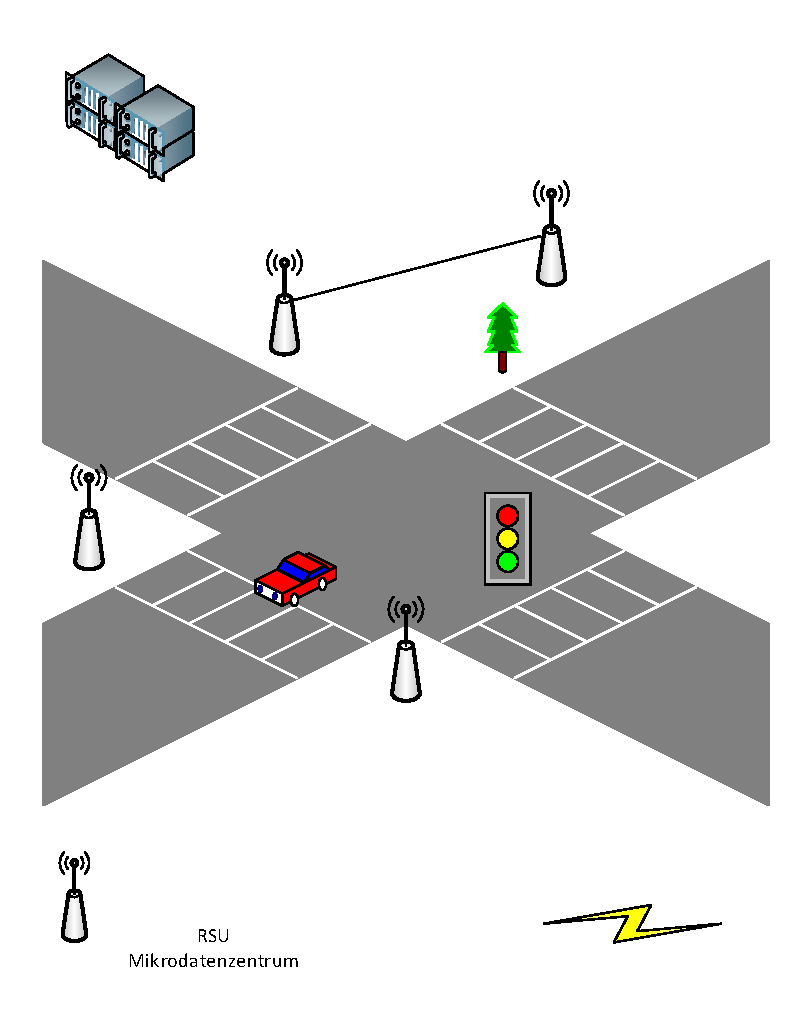
\includegraphics[scale=0.6]{strasse.pdf}
	\caption{eine Grafik ohne Sinn und Verstand}
	\label{img:grafik-dummy}
\end{figure}
\newpage

\begin{thebibliography}{1}

\bibitem{IEEEhowto:kopka}
Michael Jarschel, Thomas Zinner, Tobias Hoßfeld, Phuoc Tran-Gia, and Wolfgang Kellerer \emph{Interfaces, attributes, and use cases: A compass for SDN}, Communications Magazine, IEEE, 2014.

\bibitem{IEEEhowto:kopka}
Mohammad A. Salahuddin, Ala Al-Fuqaha, Mohsen Guizani \emph{Software Defined Networking for RSU Clouds in support of The Internet of Vehicles}, IEEE Internet of Things Journal, VOL. X, NO. X, November 2014.

\bibitem{IEEEhowto:kopka}
Mohammad A. Salahuddin, Ala Al-Fuqaha, Mohsen Guizani and Soumaya Cherkaoui \emph{RSU Cloud and its Resource Management in
support of Enhanced Vehicular Applications}, Globecom 2014 Workshop - Cloud Computing Systems, Networks, and Applications, 2014.

\end{thebibliography}

\end{document}


